\section{Grundlagen}\label{sec:grundlagen}
Dieses Kapitel soll einen grundlegenden Überblick über die zwei wichtigsten Themengebiet dieser Arbeit bieten: Digitalisierung an Schulen und Webtechnologie.

\subsection{Digitalisierung an Schulen}\label{sec:digianschulen}
Die folgenden drei Abschnitte sollen einen Einblick und eine Momentaufnahme über den Stand der Digitalisierung an deutschen Schulen (Stand 2018/2019) und den möglichen Potential von digital gestützten interaktiven Unterrichtsmethoden bieten. Ebenso wird das Thema Datenschutz an Schulen näher betrachtet.

\subsubsection{Momentaufnahme}\label{sec:technikunterricht}
Laut einer aktuellen Studie von \emph{Citrix}, sind deutsche Schüler mit Abstand am schlechtesten 
ausgestattet, was Technologie im Unterricht angeht \cite{Technisc27:online}. Die Studie hat dabei einen direkten Vergleich zwischen den vier europäischen Ländern Frankreich, Großbritannien, Niederlande und Deutschland gezogen und pro Land mehr als 1000 Schülerinnen und Schüler befragt (Niederlande 500). 22\% gaben an, gar keine Technologie im Unterricht einzusetzen, die über das Anzeigemedium Projektor hinausgeht. Innovative Technologien wie der im Abschnitt \ref{sec:problemstellung} erwähnte Einplantinencomputer \emph{Raspberry Pi}, mit denen u.A. IoT-Projekte umgesetzt werden können, stehe nur 13\% der Schülerinnen und Schülern an deutschen Schulen zur Verfügung. \\ 

Oftmals ist der normale Zustand an einer Schule jener, dass ein IT-interessierter Lehrer oder sogar der Hausmeister selbst, administrative Aufgaben die Schul-IT betreffend übernimmt, was an einem Fachpersonalmangel festzumachen sei, so Ralf Koenzen, Gründer und Geschäftsführer der \emph{LANCOM Systems GmbH} im Fachartartikel IT-Infrastrukturen an Schulen: "`Von der Kreidezeit ins digitale Zeitalter"' \cite{Koenzen2018}. Darüber hinaus seien funktionstüchtige Projektoren und Computer vielerorts Mangelware ebenso das Funknetzwerk (WLAN) nur begrenzt, wenn überhaupt, verfügbar. Dies wird auch durch die Erhebung in Abbildung \ref{fig:statistawlan} über Internet- und WLAN Verfügbarkeit in Klassenräumen gestützt. 

\begin{figure}[H]
	\centering
	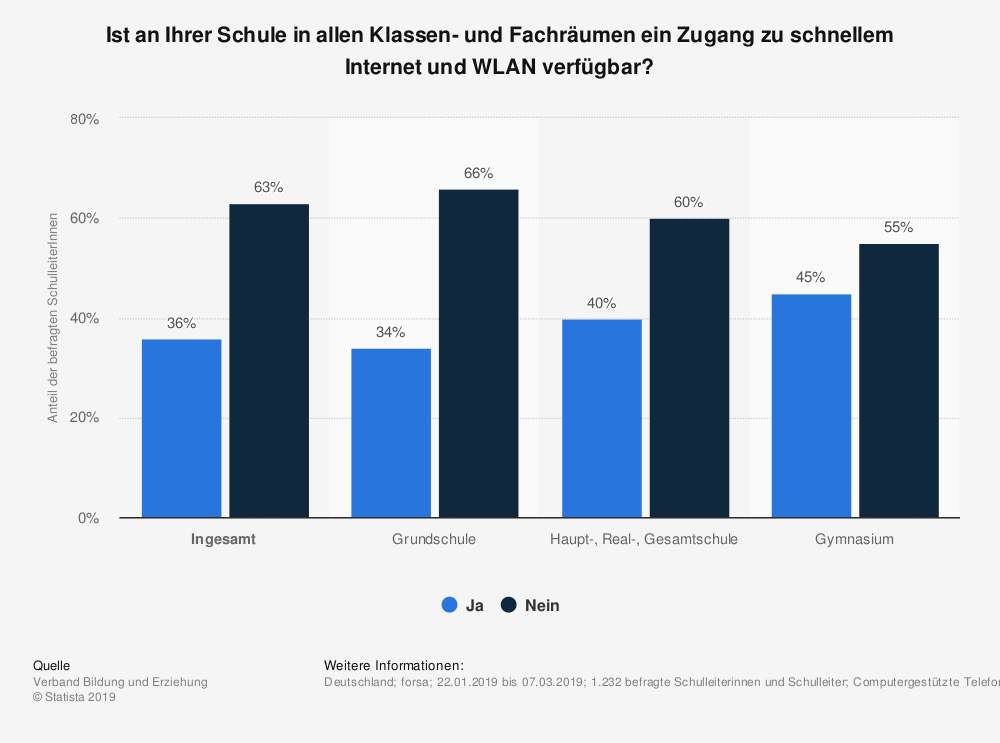
\includegraphics[width=0.9\linewidth]{bilder/statista_wlan}
	\caption[Verfügbarkeit von schnellem Internet und WLAN in Klassenräumen]{Verfügbarkeit von schnellem Internet und WLAN in Klassenräumen: Bundesweiten Erhebung zum Thema Digitalisierung an allgemeinbildenden Schulen in Deutschland. \cite{VBE2019}}
	\label{fig:statistawlan}
\end{figure}


Allerdings scheinen die ersten Barrieren durch den, in der  \hyperref[sec:einleitung]{Einleitung} dieser Arbeit bereits erwähnten, Digitalpakt Schule zu fallen. Dieser sieht vor fünf Millarden Euro in die IT-Ausstattung der deutschen Schulen fliesen zu lassen. Eine Schule mit mehr als tausend Schülern und entsprechendem Lehrkörper steht der Anforderungskomplexität an IT-Systeme eines größeren Wirtschaftsunternehmen kaum nach. Eine Ausnahme bilden hier Schulen, die auf professionelle Betreuung durch ein Systemhaus oder eigene Netzwerktechniker setzen \cite{Koenzen2018}. \\ \\ Eine interessante Alternative könnte hier das Nutzen von Cloud-Technologie sein. Cloud-basierte Netzwerkmanagementlösungen und Software-defined Networking (SDN) ist im Wirtschaftssektor bereits auf dem Vormarsch zu sein. Diese Technologien könnte Schulen dabei unterstützen den Digitalisierungsfortschritt voranzutreiben. Hierbei werden notwendige infrastrukturelle Geräte wie Access Points, Router, Switches und die nötige Verkabelung direkt vor Ort in der Schule installiert. Die Betreuung und Wartung erfolgt jedoch höchstmöglich automatisiert mit geringerem Aufwand aus der Ferne. 



\subsubsection{Ausblick digital gestützte interaktive Unterrichtsmethoden}\label{sec:interaktiveunterr}
Die erwähnte Technik im Abschnitt \ref{sec:digianschulen} macht den Einsatz von digital gestützten Interaktiven Unterrichtsmethoden möglich. Der online Lernvideo Anbieter Sofatutor hat im Jahr 2016 auf dem Educamp Leipzig Lehrerinnen und Lehrer über Software befragt, welche diese erfolgreich in ihren Unterricht integriert haben \cite{Sofatutor2019}. Neben zahlreicher Software, welche der Unterrichtsvorbereitung dient, lässt sich eine umfangreiche Liste in der Sektion "`Interaktion"' finden. Es lassen sich verschiedene Aufgabenformen ausmachen, die an einer digitalen Tafel von den Schülern gelöst werden sollen. Dies umfasst z.B. das Markieren, Sortieren, Zuordnen (Paare finden) von Bildern, Multiple-Choice Aufgaben, Brainstorming, Quiz-Anwendungen, u.v.m. Generell lässt sich feststellen, dass die Palette von Anwendungsmöglichkeiten enorm ist. Viele klassische Konzepte, die sich bereits analog interaktiv durchführen lassen konnten, stehen auch in einem digitalem Pendant bereit. Beispielsweise lassen sich Unterrichtsmethoden wie ein Lern-Quiz auch mit Papier und Stift durchführen, digitale Technik kann hier jedoch viel Arbeit abnehmen und lässt die Ausführung der Unterrichtsmethode deutlich immersiver und medial interaktiver zu. Abseits spielerischer Szenarien, kann z.B. die Mathematik Software \emph{GeoGebra} das Visualisieren von mathematischen Zusammenhängen. So Auswirkungen von anderen Werten gezeigt werden. Das Konzept "`bring-your-own-device"', welches vorsieht, dass Teilnehmende eigene Geräte mitbringen, wie z.B. ein Smartphone, steigert das Maß von Interaktivität zusätzlich. So ist es möglich, dass eine ganze Lerngruppe oder Schulklasse  an einer interaktiven Unterrichtsmethode simultan teilnimmt. Ebenso können Dozierende in einer Prüfungssituation auf Software zurückgreifen, welche die Prüfung der Teilnehmenden unterstützt und eine anschließende Auswertung der Antworten wesentlich automatisiert. An vielen Universitäten wird die Software \emph{Moodle} für diesen Zweck eingesetzt.  Zusammenfassend lässt sich feststellen, dass das Potential von digital gestützten Unterrichtsmethoden deutlich gegeben und das Angebot sowie das Potenzial der Anwendung vielfältig ist. Eine bewusste Einbettung in den Unterricht kann Dozierende unterstützen und entlasten. Als positiven Nebeneffekt lässt sich das Steigern von digitalen Kompetenzen seitens der Schülern vermerken, welche im Zuge der immer fortschreitenden weltweiten Digitalisierung eine nicht zu unterschätzende Fähigkeit ist. 
\newpage
\subsubsection{Datenschutz an Schulen}\label{sec:datenschutz}
Seit dem 25. Mai 2018 gilt die neue EU-Datenschutzverordnung, welche für alle Personen, Behörden oder sonstigen Stellen anzuwenden ist, wenn personenbezogene Daten verarbeitet werden. Dies betrifft also auch Schulen und ist sofern nichts neues, da die Datenverarbeitung und Auskunftsrechte in §64 des SchulG (Schulgesetz) im Falle des Bundeslands Berlin geregelt ist und dieser weiterhin anzuwenden ist. Neu ist allerdings, dass die Verantwortlichen für die Verarbeitung von personenbezogenen Daten weitere Aspekte berücksichtigen müssen, welche die neue Datenschutzverordnung mit sich bringt. Weiterführend sei hierzu die Quelle \cite[Datenschutz in der Schule]{Kachelriess2019} zu nennen. In diesem Zusammenhang ist es wichtig, dass auch eingesetzte Software an Schulen zu diesen Bestimmungen kompatibel sein muss, wenn diese personenbezogene Daten verarbeitet. Im Jahr 2018 an der Düsseldorfer Gemeinschaftsschule haben Unklarheiten um den Schutz von Schülerdaten dafür gesorgt, dass die Zeugnisse der rund 300 Schülerinnen und Schüler wieder per Hand geschrieben wurden. Auch die im vorherigen Abschnitt genannten Bring-your-own-device Praxis befindet sich Stand 2018 noch in einer rechtlichen Grauzone, sollten personenbezogene Daten verarbeitet werden\cite{WitmerGossner2018}. Die im Abschnitt \ref{sec:technikunterricht} genannte Auslagerung in eine Cloud könnte hier ebenfalls helfen, wenn der Cloud-Anbieter EU-Datenschutzverordnung konform arbeitet. Zur Einhaltung der gesamten Datensicherheit, ist es auf jeden Fall ratsam, wenn Cloud-Anbieter und Server ihren Standort in Deutschland haben.
Verlassen Daten alternativ gar nicht erst das Schulgelände, trägt dies ebenso positiv zum Erhalt des Datenschutzes bei.  
\newpage


\subsection{Überblick Webtechnologie}\label{sec:webbasedsoftware}
% Hier auf PDF Technische Anforderungen verweisen (Footnote?) da sehr ausführlich und gut
% Anfang Geschichtlich
In den folgenden Untersektionen \ref{sec:websoftpopular} ff. wird ein Überblick über Webtechnologie und Web-Softwareentwicklung gegeben.

\subsubsection{Popularität}\label{sec:websoftpopular}
Seit dem Erfolgskurs des Web 2.0\footnote{Web 2.0 ist ein Schlagwort, das für eine Reihe interaktiver und kollaborativer Elemente des Internets, speziell des World Wide Webs, verwendet wird. Dabei konsumiert der Nutzer nicht nur den Inhalt, er stellt als Prosument selbst Inhalte zur Verfügung. - Wikipedia.org} in den frühen 2000er Jahren, zeichnet sich zunehmend der Trend des Software-as-a-Service Geschäftsmodells ab. Dies beschreibt die Bereitstellung von Software im Internet oder durch ein lokal laufenden Servers, ohne dass Benutzende die Software selbst noch lokal installiert haben müssen. Im Jahr 2015 setzten bereits über drei Viertel von 102 befragten Unternehmen Software dieser Form aktiv im Geschäft ein \cite{TecArt-GmbH2019:online}. Viele Arten von Software können  mittlerweile in einer im Webbrowser lauffähigen Alternative substituiert werden. Ein populäres Beispiel ist die Office-Suite \emph{Google Docs} der Firma \emph{Google inc.} Hier lassen sich Textverarbeitung, Tabellenkalkulation und das erstellen von Präsentationen ohne Installation und direkt im Webbrowser des Benutzenden ausführen. Ein anderes Beispiel ist die Web-Software \emph{Photopea} welche ebenfalls komplett im Web-Browser ausgeführt wird und dem nur lokal installiert ausführbaren Bildbearbeitungsprogramm \emph{Photoshop} der Firma \emph{Adobe inc.} sehr nahe kommt. Im Vergleich zu lokal installierter Software ist die Bereitstellung von Web-Software einfacher, da solange ein moderner Webbrowser lauffähig ist, das Betriebssystem des Client-Computers zu vernachlässigen ist. Ebenso stellt potente Hardware keine zwingende Voraussetzungen, da etwaige rechenintensive Aufgaben auf der Serverseite getätigt werden können oder hier eine Balance zwischen Client und Server angestrebt werden kann. \\ 

\subsubsection{Intranet und Internet}\label{sec:intranetundinternet}
% Detailgrad so sinnvoll?
% Unterschied und Gemeinsamkeit klar machen
% Hier kommunikation erklären! Protokolle und OSI schicht!
Einfach ausgedrückt, ist das Internet ein Netzwerk von Computern, welche weltweit miteinander vernetzt sind. Seine Anfänge lassen sich auf das Ende der 1960er in den USA datieren, als die DARPA (Defense Advanced Research Projects Agency) eine weltweite Verknüpfung von Datennetzen anstrebte. Das hier draus resultierende ARPANET (Advanced Research Projects) kann als Ursprung angesehen werden. Dabei beschreibt der Begriff Internet streng genommen ein 'interconnected network', also ein international vernetztes Netzwerk, ohne dabei die Hardware- und Netzwerktechnologie genauer zu beschreiben \cite{Safran2011}.  \\ 
Die wohl populärste Anwendung des Internets ist das World Wide Web, welche gegen das Jahr 1989 von einer Forschungsgruppe rund um Sir Tim Berners-Lee ins Leben gerufen wurde und heute oftmals als Synonym für das gesamte Internet sprachlich genutzt wird. \\ 

In unser heutigen globalisierten Welt lässt sich das Internet mitsamt World Wide Web nicht mehr wegdenken und ist ein integraler Bestandteil der Kultur und Struktur des weltweiten Informationsaustausches.
 \\ \\
 Das Intranet beschreibt analog dazu ein lokal abgeschlossenes Netzwerk von Computern, bspw. innerhalb eines Unternehmens. Dabei endet ein Intranet an seinen Grenzen und ein Gateway fungiert als Übergabepunkt ins Internet (siehe Abbildung \ref{fig:intranetinternet}). Die Vernetzung der Endgeräte erfolgt kabelgebunden (LAN) oder kabellos (WLAN). Die Kommunikationsgeschwindigkeit innerhalb eines Intranets sind i.d.R. deutlich höher als im Internet, da Daten nicht erst nach außen an einen Internet Service Provider übermittelt werden müssen. Ein Intranet funktioniert unabhängig vom öffentlichem Internet (erhöhte Ausfallsicherheit), ist nicht öffentlich zugänglich und bietet oft andere oder zusätzliche Funktionen \cite{Intranet62:online}. 
 
 \begin{figure}[H]
 	\centering
 	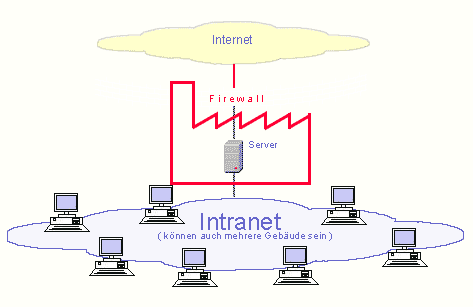
\includegraphics[width=0.8\linewidth]{bilder/intranetinternet}
 	\caption[Schematische Darstellung Intranet und Internet]{Schematische Darstellung Intranet und Internet \cite{intranet2019}}
 	\label{fig:intranetinternet}
 \end{figure}
 

 \subsubsection{Client-Server Modell}\label{sec:clientservermodell}
 Das Client-Server Modell beschreibt das Prinzip der Kommunikation zwischen zwei Teilnehmern innerhalb eines Netzwerks. Grundlegend unterscheidet das Modell hierbei zwischen einer Anbieterseite (Server) und einer Benutzerseite (Client). Der Client betreibt auf seinem Endgerät (Computer, Smartphone, etc.) eine Client-Software mit der die Verbindung zum Server aufgebaut wird. Im Fall des WWW (siehe \ref{sec:www}) ist dies in den meisten Anwendungsszenarien ein Webbrowser. Der Client fordert dabei eine Ressource an, welche auf dem Server vorliegt oder dort speziell für die Anfrage des Clients generiert wird (siehe auch Sektion \ref{sec:webanwenservices}). Das Client-Server Modell sieht vor, dass immer der Client die Verbindung aufbaut, nie andersherum \cite{ElektronikKompendium.de:online}. Die Anfrage des Clients wird \emph{Request} genannt, die Antwort des Servers \emph{Response} oder \emph{Reply}, welche bei ausreichender Berechtigung des Clients auch Daten enthält. 
 Server-Computer sollen rund um die Uhr erreichbar sein, während Client-Endgeräte auch abgeschaltet werden können, ohne die Integrität des Netzwerks zu beeinflussen. 
  % Vergleich zu anderen Modellen?
 
\subsubsection{Kommunikation}\label{sec:kommunikation}
Die Kommunikation im Internet und Intranet erfolgt über Protokolle. 
Ein Protokoll kann als ein Satz von Kommunikationsregelvorschriften \cite{Safran2011} verstanden werden, welche den Netzwerkverkehr auf unterschiedlichen Schichten reglementieren. 
Diese Schichten werden im \emph{OSI-Modell} (Open System Interconnection) der \emph{ISO} (International Standardization Organisation), der internationalen Standardisierungsorganisation beschrieben. 
\\ 
Das \emph{ISO-OSI-Modell} ist dabei in sieben Schichten eingeteilt, während die Erste als physikalische Schicht definiert ist und die Siebte als Anwendungsschicht. Protokolle sind dabei jeweils nur über Protokolle benachbarter Schichten in Kenntnis gesetzt. Es lässt sich grob in anwendungsorientierte Schichten (1 bis 4) und transportorientierte Schichten (5 bis 7) unterteilen. Die im Rahmen dieser Arbeit genutzten Webtechnologien nutzen kommunikativ nur anwendungsorientierte Schichten des \emph{ISO-OSI Modells}.



% Begriff Internet
\subsubsection{World Wide Web}\label{sec:www}
Das \emph{World Wide Web} (WWW) ist die wohl populärste Anwendung des Internets~\cite{Safran2011} und wird oftmals fälschlicherweise als Synonym für das gesamte Internet genannt. Das WWW ist eine Sammlung von verteilten Dokumenten, welche sich gegenseitig über sog. Hyperlinks referenzieren und von Web-Servern zur Verfügung gestellt werden. Auf der Client Seite (siehe \ref{sec:clientservermodell}) stellt der Web-Browser die wichtigste Software da. Mit ihr werden Web Server angesprochen (Request) und Antworten (Response) für den Nutzenden dargestellt. Die wichtigsten sprachlichen Komponenten des WWW sind: \\ 
\begin{itemize}
	\item \textbf{HTML:} Hypertext Markup Language - eine reine Beschreibungssprache, welche Hypertext Dokumente durch Tags codiert. 
	\item \textbf{CSS:} Cascading Style Sheet - Eine Stylesheet-Sprache, welche das äußere Erscheinungsbild von Hypertext Dokumenten beschreibt
	\item \textbf{JS:} JavaScript: Eine Skriptsprache, welche u.A. Interaktion sowie Dynamik hinzufügt und clientseitig interpretiert wird. 
\end{itemize}
Die Techniken des WWW können auch lokal im Intranet genutzt werden. 
Das zur Verständigung zwischen Client und Server genutzte Protokoll (siehe \ref{sec:kommunikation}) ist das \emph{Hypertext~Transfer~Protocol} (HTTP) bzw. in verschlüsselter Form \emph{Hypertext~Transfer~Protocol~Secure} (HTTPS), da eine Übermittlung im Klartext nicht immer wünschenswert ist. HTTP/HTTPS ist ein Zustandsloses Protokoll, das bedeutet dass jede Anfrage unabhängig voneinander geschieht und betrachtet wird. Dies und die Tatsache, dass jede Anfrage von der Client-Seite aus gestartet werden muss (siehe \ref{sec:clientservermodell}), stellen oftmals Hürden für die Entwicklung von Webanwendungen und Webservices da. Techniken wie \emph{Cookies} und \emph{Sessions}, sowie das wiederholte Abfragen von aktualisierten Daten seitens des Clients wirken hier entgegen. \emph{Cookies} stellen persistent gespeicherte Daten auf der Client-Seite da, mit deren Hilfe der Webserver einen Client eindeutig zuordnen kann. Bei einer \emph{Session} sendet der Client bei jeder Anfrage eine eindeutige ID an den Server. Im Normalfall endet eine Session beim Beenden des Webbrowser, während Cookie-Dateien eine längere Lebensdauer besitzen.      
%
\subsubsection{Webanwendungen und Webservices}\label{sec:webanwenservices}
Im Laufe der Entwicklung des WWW (siehe \ref{sec:www}) stieg der Anspruch vom reinen Anbieten statischer Dokumenten in Richtung dynamischer Inhalte, welche einer Programmlogik folgend von einem Webserver für jede Anfrage generiert werden. Web\-anwendungen sind Computerprogramme, welche auf einem Webserver ausgeführt werden und den Webbrowser des Clients als Schnittstelle nutzen \cite{Safran2011}. Dies bietet den großen Vorteil, dass etwaige Anpassungen von Programmlogik nur serverseitig erfolgen müssen und jeder Client mit Webbrowser als Benutzerschnittstelle ausreicht. \\ \\
Webservices sind eine spezialisierte Art von Webanwendung. Der Fokus hier liegt auf dem Bereitstellen von Daten für andere Applikationen, welche die gewonnen Daten selbst auswerten und dem Nutzenden bereitstellen. Dies geschieht i.d.R. über eine einheitlich beschriebene Schnittstelle (API - \emph{Application Programming Interface}), über welche fremde Applikationen angefragte Daten abrufen können. Der Austausch der Daten erfolgt hier meist über Formate wie JSON (\emph{JavaScript Object Notation}) oder XML (\emph{Extensible Markup Language}), da Aussehen und Lesbarkeit der Daten irrelevant sind und somit eine Ausgabe in HTML nicht von Nöten ist. \\
Bei der Implementierung eines Webservices bieten sich folgende zwei technologische Arten der Umsetzung an: \\ \\
\textbf{SOAP/WSDL}: Hier werden Nachrichten über das \emph{Simple Object Access Protocol} (SOAP) ausgetauscht und deren Beschreibung über die \emph{Web Services Description Language} (WSDL) definiert. Anfrage- und Antwortformat der Daten ist XML, eine Auszeichnungssprache, welche HTML sehr ähnelt aber deutlich allgemeiner ist. XML kann also mehr als Regelwerk verstanden werden, mit dessen Hilfe Entwickelnde ihre eigene hierarchische Beschreibung einer Datenstruktur vornehmen können. XML und HTML leiten sich bei der von der SGML (\emph{Standard Generalized Markup Language}) ab, welches ihre Ähnlichkeit zusätzlich begründet \cite{XMLHTMLU88:online}. \\

 
\textbf{REST}: Representational State Tranfer - Hier kann jede einzelne Funktion des Webservices über eine jeweils zugeordnete URL (\emph{Uniform Resource Locator}) abgerufen werden, umgangssprachlich als Webadresse bekannt. Das WWW selbst kann als REST-Webservice verstanden werden \cite{Bayer2002:online}. \\ 

\subsection{Websockets}\label{sec:websockets}
Bezugnehmend auf die Problematik, welche durch die Kommunikationsstrategie über das http-Protokoll entsteht (siehe Sektion \ref{sec:www}), wirken \emph{Websockets} dieser entgegen. Als Kommunikationskanal verknüpft ein \emph{Websocket} Server und Client. Zwar muss die Kommunikation zunächst über den Client initiiert werden, bleibt dann jedoch bestehen und der Server kann diese nutzen um aktiv neue Daten zu emittieren. Ein Nachteil ist jedoch, dass im Gegensatz zum http-Protokoll hier auch Daten hin- und hergeschickt werden, wenn dies eventuell nicht gewünscht ist~\cite{neumann2015entwicklung}, was insbesondere bei mobilen Applikationen kritisch sein kann. Ein generellen Vorteil bieten \emph{Websockets} auch in Sachen Performanz, da das Protokoll, ist erst einmal eine Verbindung zustande gekommen, deutlich schlanker ist. \\ Die folgende Abbildung \ref{fig:socketsrest} zeigt einen Performanz Vergleich in Anbetracht des zusätzlichen \emph{Payloads} von REST- und \emph{WebSocket} Nachrichten. 

\begin{figure}[H]
	\centering
	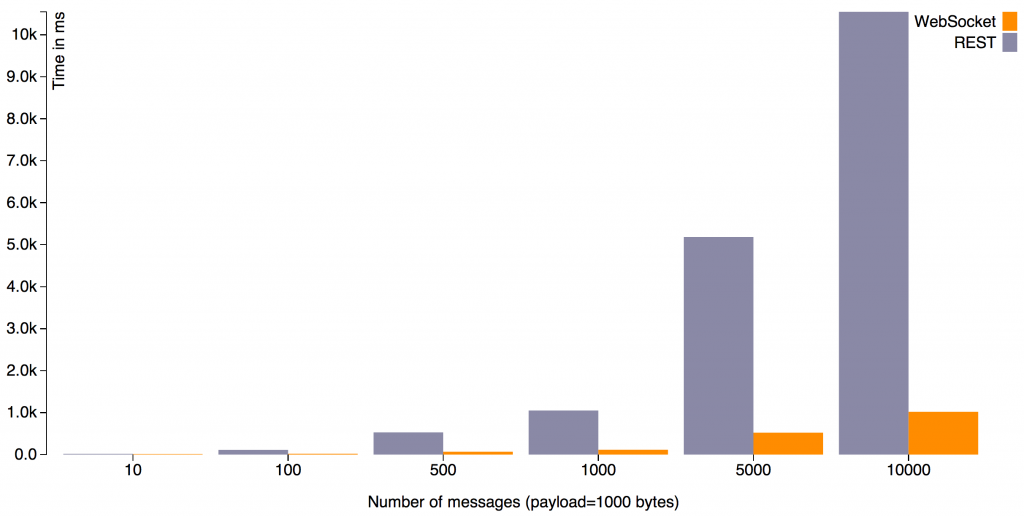
\includegraphics[width=0.9\linewidth]{bilder/websocket-rest-messages}
	\caption[Performanzvergleich REST versus WebSockets]{Performanzvergleich REST versus WebSockets \cite{Gupta2014}: \\ Benötigte Zeit um N Nachrichten einer konstanten Nachrichtengröße zu verarbeiten.}
	\label{fig:socketsrest}
\end{figure}

\subsection{Webapplikationsentwicklung}\label{sec:softwareentwicklung}
Dieses Kapitel beleuchtet wesentliche Begriffe hinsichtlich der Entwicklung von Webapplikationen.
Webanwendungen und Webservices können unter diesem Begriff zusammengefasst werden.
\\ 
\subsubsection{Web-Application-Frameworks} \label{sec:wafs}
Bei der Entwicklung von Webapplikationen wird oftmals auf Frameworks, spezifischer Web-Application-Frameworks (WAF) zurückgegriffen. 
Ein WAF bezeichnet ein Programmgrundgerüst, welches als Grundlage im Implementierungsprozess zum Einsatz kommt \cite{Ionis2019:online}. Dies erleichtert die Entwicklung ungemein, da auf bereits vorgefertigte Ansätze und Programmbausteine zurückgegriffen werden kann. Diese WAFs reflektieren zumeist auch Modelle und Prinzipien, was einen gewissen Grad an Konformität gewährleistet und das Verständnis für den Quellcode erhöht.
Ein für Frameworks bekanntes Paradigma stellt das Umsetzungsparadigma \\
\textbf{Inversion of Control} (IoC), z. Dt. Umkehrung der Steuerung dar, welches u.a. auch in der objektorientierten Programmierung Anwendung findet.
Hierbei wird eine Funktion/Unterprogramm bei der Hauptprogrammbibliothek registriert und von dieser zu einem späteren Zeitpunkt aufgerufen. Dies ist umgangssprachlich auch als 'Hollywood'-Prinzip bekannt ("`Don't call us! We call you"' z. Dt. "`Ruf nicht uns an! Wir rufen dich an!"'). Das Framework behält also die Programmflusssteuerung bei. 
  Ein Nachteil, der durch den Einsatz von eines WAFs bedingt ist, stellt die Einschränkung der Freiheit während des Implementierungsprozesses dar. Dieser wird jedoch billigend in Kauf genommen, da sich ein Reduktion des Zeit- und Kostenaufwands erhofft wird. Die Wahl des richtigen WAFs ist ein wichtiger Entschcheidungsprozess, bei dem mehrere Faktoren beachtet werden müssen, wie z.B. benötigte Einarbeitungszeit und Lizenzen.

\subsubsection{Serverseitiger Ansatz}\label{sec:serverseitgeransatz}
Anknüpfend an Sektion \ref{sec:webanwenservices} sind Webapplikationen Software, welche serverseitig ausgeführt werden, wobei der Webbrowser eines Nutzenden als Benutzerschnittstelle dient. Eine Webapplikation kann jedoch auch clientseitig implementiert werden, wie in Sektion \ref{sec:clientseitigeransatz} beschrieben. \\ 
Serverseitige Webapplikationen verfolgen oftmals den \emph{Multi-Page} Ansatz, das heißt pro Anfrage (Request) wird dem Client (Webbrowser) ein anderes Dokument  übergeben. Wichtige Programmiersprachen für den Ansatz sind \emph{php}, \emph{Ruby}, \emph{Python}, \emph{Java} und auch \emph{JavaScript}. Letzteres kam zuvor nur auf der Clientseite zur Anwendung. \\
Die \textbf{Model - View - Controller} Architektur (MVC) ist die vorherrschende Architektur, auf welche sich der Großteil der serverseitigen WAFs stützen.
Hierbei wird die Programmlogik klar in drei große Bestandteile unterteilt: \\ \\
\textbf{Model}: Das Model oder z. Dt. Modell (im restlichen Teil der Ausarbeitung \emph{Model} geschrieben) beschreibt eine Datenstruktur an sich. In einem Webshop wären dies z.B. die Produkte und deren Eigenschaften wie ID, Name, Preis usw. \\
\textbf{View}: Sie beschreibt die reine Ansicht eines \emph{Models}. In einem Webshop wäre dies z.B. die Detailseite eines Produkts. \\
\textbf{Controller}: Der Controller dient als Bindeglied zwischen \emph{Model} und \emph{View}. Er handelt ankommende \emph{Requests} (Anfragen) ab und übergibt der \emph{View} aus dem Modell die notwendigen Daten. \\ 
Neben der MVC Architektur existieren weitere, andere Architekturen und Ableitungen der MVC Architektur, wie z.B. der im \emph{Django} WAF genutzten \emph{Model - View - Presenter} Architektur. \\
Die folgende Tabelle \ref{tab:servwaf} zeigt einen groben Überblick über bekannte WAFs, welche den serverseitigen Multi-Page Ansatz verfolgen \cite{TopWebDe0:online}. 

\begin{table}[H]
	\centering
	\caption{Überblick einiger serverseitiger Web-Application-Frameworks}
	\label{tab:servwaf}
	\begin{tabularx}{0.8\textwidth}{llX}
		\textbf{Name} & \textbf{Sprache} & \textbf{Architektur}   \\ 
		\toprule
		Symfony & php & Model - View - Controller \\
		\rowcolor[HTML]{EFEFEF} 
		Laravel	& php & Model - View - Controller  \\ 
		Phalcon	& php & Model - View - Controller   \\
		\rowcolor[HTML]{EFEFEF}  
		Codeigniter & php & Model - View - Controller \\
		Django & Python & Model - View - Presenter \\	
		\rowcolor[HTML]{EFEFEF} 	
		Ruby on Rails & Ruby & Model - View - Controller \\
		\hline 
	\end{tabularx} 
\end{table}


Aus der Tabelle lässt sich eine starke Popularität der Programmiersprache \emph{php} ableiten und deren auf dieser Sprache basierenden WAFs. Die Tabelle stellt keinen Anspruch auf Vollständigkeit, da noch unzählig viele andere serverseitige WAFs existieren. Ebenso wurde das WAF \emph{ExpressJS}, welches auf der serverseitigen Plattform \emph{NodeJS} basiert, bewusst nicht mit in die Tabelle aufgenommen, da dies ein Sonderfall darstellt. Diese Thematik wird in Kapitel \ref{sec:konzept} ausführlich behandelt. 
%Hier über NodeJS und PHP quatschen!
\subsubsection{Clientseitiger Ansatz}\label{sec:clientseitigeransatz}
 Das Programmiermodell des WWW, welches durch die Architektur des HTTP geprägt ist, wird bei der Entwicklung von Webapplikationen übernommen. Dies sieht eine Anfrage immer seitens des Clients vor (siehe auch Sektion \ref{sec:www}). Dies schränkt das Ausmaß von Interaktion und generieren von dynamisch ladenden Webseiten ein. 
 Der clientseitige Ansatz der Webapplikationsentwicklung kommt meistens bei sog. Single-Page-Applikationen zur Anwendung. Hierbei wird o.g. Problem damit umgangen, indem bei Aufruf einer Internetseite die gesamte HTML Benutzeroberfläche inklusive Programmlogik in Form von JS Code als Ganzes an die Client übergeben wird. Dies bietet den großen Vorteil, dass die Logik nun auf dem Client ausgeführt wird und dieser dynamisch Daten nachladen bzw. Anfragen kann. Oftmals ändert sich auf einer Single-Page Applikation die Webadresse in der Adresszeile des Browsers nicht. Die ganze Applikation läuft also auf einer einzelnen Website ab, die sich dynamisch ändert. Dieses dynamische Nachladen von Inhalten wird \textbf{AJAX} - \emph{Asynchronous JavaScript and XML} genannt.  Die einzig nativ unterstützte Programmiersprache seitens der Webbrowser ist \emph{JavaScript} und daher vorherrschend \cite{Safran2011}.
 Jeder moderne Webbrowser hat einen JS Interpreter integriert. Über Plugins können zwar auch andere Sprachen genutzt werden, in Form von \emph{Java-Applets} (Programmiersprache dort \emph{Java}) oder das früher sehr populäre \emph{Flash} des Unternehmens \emph{Adobe}, welches \emph{ActionScript} als Programmiersprache nutzt. Beides gilt aber Stand 2019 als veraltet und der Einsatz derartigen Technologien wird nicht empfohlen. %Nachweis nötig?
Es gibt sehr viele JavaScript WAFs und Bibliotheken, zu den bekanntesten zählen: \\ \\ 
% hier noch bisschen mehr vielleicht
 \textbf{Angular} ist ein clientseitiges \emph{JavaScript} WAF, entwickelt und bereitgestellt von dem Unternehmen \emph{Google inc}. Es hat vergleichsweise eine steile Lernkurve und setzt etwas Einarbeitungszeit voraus. \\ \\
 \textbf{React} ist streng genommen kein WAF, sondern lediglich eine JS Bibliothek. Es bietet aber über Erweiterungen die Möglichkeit, wie ein WAF genutzt werden zu können, was seine Flexibilität noch erhöht. Entwickelt und Betrieben wird \emph{React} von der Firma \emph{Facebook inc.} \\ \\
 \textbf{Vue} ist ein clientseitiges \emph{JavaScript} WAF, ursprünglich entwickelt von dem Entwickler Evan You. Es gilt als einfacher zu erlernen als \emph{Angular} und ist sehr flexibel. \\ 
 
 
 Das Entwickeln von clientzentrischen JS Anwendungen ist mittlerweile so fortgeschritten, dass oftmals beim Nutzenden ein Gefühl entsteht, es würde ein lokal installiertes Programm ausgeführt werden. Populäre Beispiele wäre das in Kapitel \ref{sec:zielsetzung} erwähnte \emph{Google Docs}, welches eine voll umfassende Textverarbeitungslösung im Browser bietet. Derartige Applikationen werden \emph{Rich Internet Application} (RIA) genannt.
 

%Hier vor allem über Javascript quatschen!
\subsubsection{Hardware Anforderungen}\label{sec:hardware}
Auf der \textbf{Serverseite} ist der Anspruch an die Hardware sehr abhängig vom gewünschten Anwendungsfall und benötigter Skalierbarkeit. Das beliebte Server \emph{Linux} Derivat \emph{Debian} benötigt bspw. mindestens 128~Megabyte Ram-Speicher und 2~Gigabyte Festplattenspeicher. Es ist aber durchaus möglich mit noch sehr viel weniger potenter Hardware ein Server zu betreiben \cite{dpakt2019:online}. 
Für den Einsatz in einzelnen Unterrichtsklassen an Schulen würde ein \emph{Raspberry Pi 3} Einplantinencomputer bereits genügend Leistung für Webanwendungen und einen günstigen Anschaffungspreis bieten. Auch besitzen bereits 67\% der 10 bis 11 jährigen Jugendlichen Smartphones \cite{Statista2017:online}, welche ebenfalls genug Leistung für Webanwendungen aufweisen und als Clients genutzt werden können. \\ 
\subsubsection{Vergleich zu anderen Entwicklungsansätzen}\label{sec:vorundnachteileweb}
Der klassische Ansatz der Software Entwicklung wäre das Implementieren eine Desktop-Anwendung, welche lokal
auf dem Computer des Anwendenden installiert wird. Typischerweise wird die Software programmiert und anschließend von einem Compiler in Maschinencode übersetzt bzw. von einer Laufzeitumgebung zur Ausführung interpretiert. Die Software wird also normalerweise auf dem Computer installiert und an die Gegebenheiten des Betriebssystems angepasst. Dies hat den Vorteil bei Bedarf sehr hardwarenah und performant entwickeln zu können, was durch das vorherige kompilieren des Codes in Maschinencode begünstigt wird. Nachteilig ist es jedoch, dass die Software zunächst überhaupt installiert werden muss. Eine noch vergleichsweise neue aber vielversprechende Webtechnologie ist in dieser Hinsicht \emph{Webassembly} (WASM). Dies ist ein Bytecode, welcher neben der virtuellen JS-Maschine im Webbrowser ausgeführt wird und aus Programmiersprachen wie \emph{C}, \emph{C++} oder \emph{Rust} kompiliert wird. Dies soll die Monopolstellung von JS als einzig ausführbare Sprache im Webbrowser adressieren und vor allem auf rechenintensiven Anwendungsgebieten einen Vorteil erbringen \cite{Stueckler2018}. \\  Die folgende Tabelle \ref{tab:vergleichwebdesk} vergleicht Web- und Desktopapplikationen hinsichtlich gängiger Kriterien.

\begin{table}[H]
	\centering
	{\footnotesize
	\caption{Vergleich von Web- und Desktopapplikationen \cite{TecArt-GmbH2019:online}}
	\label{tab:vergleichwebdesk}
	\begin{tabularx}{\linewidth}{l  X  X}
		\textbf{Kriterium} & \textbf{Webapplikation} & \textbf{Desktopapplikation}   \\ 
		\toprule 
		Struktur & Modularer Aufbau & Meist als Gesamtpaket vertrieben \\
		\rowcolor[HTML]{EFEFEF} 
		Verfügbarkeit & Weltweit dank Internet, \newline lokal eingeschränkt möglich & Nur bei lokaler Installation verfügbar \\ 
		
		Installation	& Nicht erforderlich & Erforderlich   \\ 
		\rowcolor[HTML]{EFEFEF} 
		Speicher & Kein Zusätzlicher Speicher benötigt & Installation benötigt Speicherplatz \\
		
		Updates & Live-Aktualisierung möglich & Teil- oder Neuinstallation notwendig \\		
		\rowcolor[HTML]{EFEFEF} 
		Teamarbeit & Zeitgleiches und schnelleres Arbeiten leicht möglich & Teamarbeit nur über Synchronisation möglich \\
		
	\end{tabularx}
	}
\end{table}

